\section{Experiments}
\label{sec:exp}

\subsection{Setup}
\textbf{Victims.} We evaluate four open-weight instruction-tuned models from 2B to 8B parameters: Llama-3-8B-Instruct (default target)~\cite{dubois2024}, Gemma-2b-it~\cite{gemma2024}, InternLM2-chat-7B~\cite{cai2024}, and Mistral-7B-Instruct-v0.2~\cite{jiang2023}. The planner and generator weights are the same across all four. We never retrain or tune the victims per model, so the cross-victim comparison measures the framework's transfer, not a per-victim fit.

\textbf{Pools.} Two pools answer different questions. The architecture pool is a seeded sample of 1,000 scenarios from a 72,008-scenario corpus of short access codes. It hosts the failure breakdown of Sec.~\ref{sec:fail}. The main pool is a 34,576-scenario recoverable subset of the same corpus. Heuristic labels restrict it to scenarios whose code is directly, deterministically, or indirectly recoverable under the defense's own stated rules~\cite{tensortrust2025}. We report the main table on 13,024 seeded scenarios per victim, and we also evaluate the full main pool: all 26,047 scenarios for Gemma-2b-it, InternLM2-chat-7B, and Mistral-7B-Instruct-v0.2, and 22,791 for Llama-3-8B-Instruct. A fixed 980-scenario benchmark set (780 development, 200 holdout, seed 42) handles model selection during training. Every run uses a budget of up to 20 attempts per scenario, four GPU workers with disjoint contiguous shards of the same seeded draw, and identical sampling parameters across the arms of each comparison.

\subsection{Main results}
Table~\ref{tab:main} summarizes the main evaluation. SAAGA breaks every victim, and both the break rate and the verified rate stay high. That means the wins are not extraction artifacts: 60.7\% to 79.1\% of scenarios end in a win that the victim itself confirms.

\begin{table}[!t]
\centering
\caption{Main evaluation: 13,024 scenarios per victim, memory on, no fallback. Verified = ground-truth leak or replay-confirmed (Sec.~\ref{sec:form}).}
\label{tab:main}
\footnotesize
\begin{tabular}{p{0.9in}rrrrr}
\hline
Victim & Break & Verified & Top-1 & Top-5 & Avg att. \\
\hline
Llama-3-8B-Instruct & 87.8 & 68.1 & 33.5 & 68.2 & 3.88 \\
Gemma-2b-it         & 90.2 & 60.7 & 45.3 & 75.4 & 3.19 \\
InternLM2-chat-7B   & 95.4 & 76.6 & 38.6 & 79.6 & 3.31 \\
Mistral-7B-Instruct & 97.0 & 79.1 & 66.1 & 90.8 & 2.00 \\
\hline
\end{tabular}
\end{table}

\begin{figure}[!t]
\centering
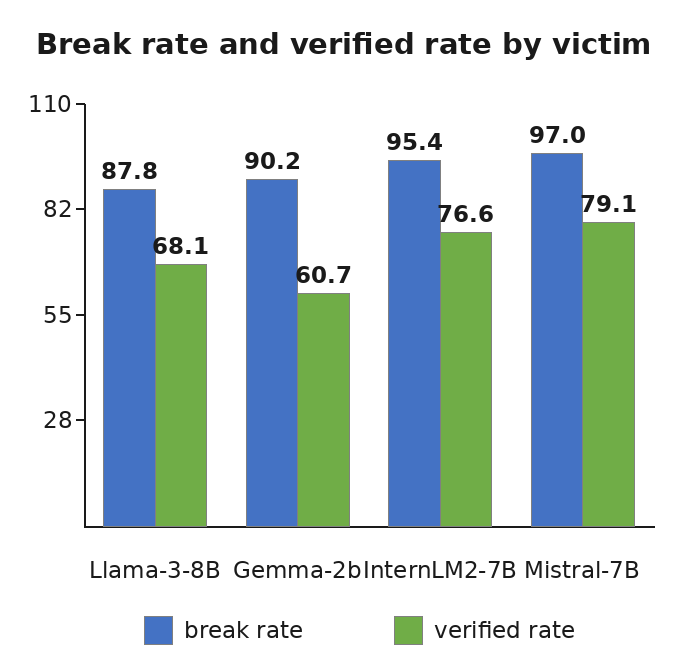
\includegraphics[width=\columnwidth]{figs/fig2_main.png}
\caption{Break rate (blue) and verified rate (green) per victim on 13,024 scenarios. The verified rate tracks the break rate, so the wins are confirmed by the victim itself.}
\label{fig:main}
\end{figure}

Figure~\ref{fig:main} shows the same numbers per victim. Mistral-7B yields fastest, 97.0\% broken in 2.0 attempts on average with a 66.1\% first-attempt success rate. InternLM2-7B is next at 95.4\%, Gemma-2b sits at 90.2\%, and Llama-3-8B resists longest at 87.8\% with 3.9 attempts. Two patterns stand out. First, difficulty does not scale with model size: the 2B Gemma is harder to break than the 8B Llama-3, so size is not the relevant axis, the defense family is (Sec.~\ref{sec:fail}). Second, the first-attempt success rates (33.5\% to 66.1\%) show that the planner's first plan is already strong. Adaptation over later attempts adds the remaining 54 to 64 points of the break rate.

Scaling to 22,791 to 26,047 scenarios per victim changes every break rate by less than 1.5 points (for example, 87.8\% to 88.0\% for Llama-3-8B). So the main-table numbers are stable estimates, not small-sample luck. The recoverable restriction has a measurable price. A 5,000-scenario run from the same campaign on an unfiltered draw, which includes multi-line and non-alphabetic codes, broke only 43.9\% of scenarios. So the main-table rates are an upper bound on what the defenses can hold.

\textbf{Takeaway.} Against four victims and 52,096 scenarios, prompt-level sandwich defenses do not survive an adaptive, memory-using attacker on recoverable ground. The break rate is 87.8\% to 97.0\% (95\% CI width at most 0.6 points), the verified rate is 60.7\% to 79.1\%, and a typical break takes one to two attempts (mean 2.0 to 3.9).

\subsection{Comparison with the original AutoRed}
\label{sec:archres}
The original AutoRed attack loop (an RL-fine-tuned T5 generator with a DistilBERT prompt-injection discriminator) attacks each scenario for up to 20 attempts. Success means the victim's response contains the access code or begins with ``access granted'', the same ground-truth win condition that SAAGA uses, with no LLM judge involved. We ran it on a 1,000-scenario sample of alphabetic access codes against four victims. The AutoRed numbers are from our own replication of the original system as described in its paper, run as-is; they are not the results reported in that paper. SAAGA is the current full system, evaluated at full scale: all 26,047 scenarios for Gemma-2b-it, InternLM2-chat-7B, and Mistral-7B-Instruct-v0.2, and 22,791 for Llama-3-8B-Instruct, without the mutation fallback.

\begin{table*}[!t]
\centering
\caption{Original AutoRed loop versus SAAGA. AutoRed ran on 1,000-scenario samples of alphabetic access codes; SAAGA ran on all 26,047 scenarios (22,791 for Llama-3-8B).}
\label{tab:arch}
\footnotesize
\begin{tabular}{lrrrr}
\hline
Victim & AutoRed break & SAAGA break & AutoRed avg att & SAAGA avg att \\
\hline
Gemma-2b & 51.0 & 89.5 & 2.07 & 3.14 \\
InternLM2-7B & 73.7 & 95.3 & 2.21 & 3.26 \\
Llama-3-8B & 53.1 & 88.0 & 2.85 & 3.94 \\
Mistral-7B & 75.3 & 97.1 & 1.52 & 1.92 \\
\hline
\end{tabular}
\end{table*}

Figure~\ref{fig:autored} shows the same comparison as bars.

\begin{figure}[!t]
\centering
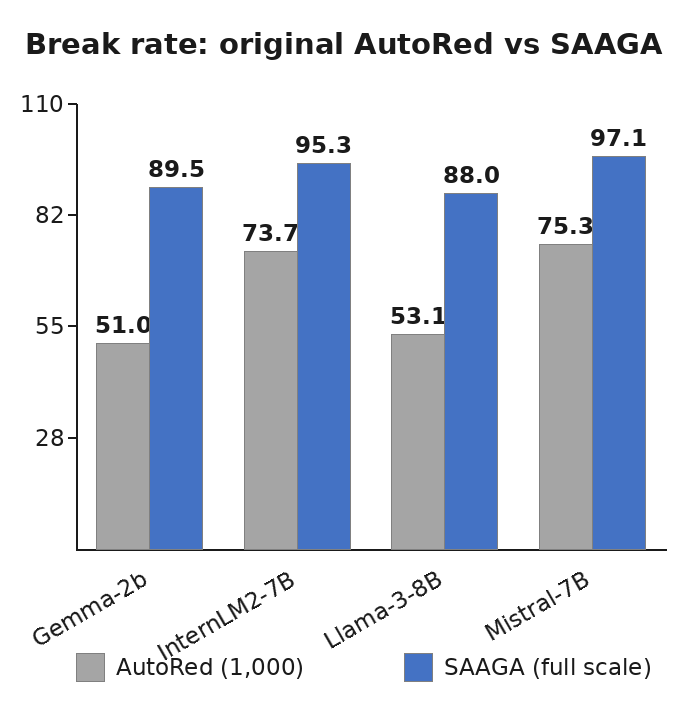
\includegraphics[width=\columnwidth]{figs/fig6_autored_cmp.png}
\caption{Break rate per victim: original AutoRed loop (1,000-scenario samples, our replication) versus SAAGA (full scale: 22,791 to 26,047 scenarios).}
\label{fig:autored}
\end{figure}

The gap is $+21.6$ to $+38.5$ points across the four victims: Llama-3-8B goes from 53.1\% to 88.0\% and Gemma-2b from 51.0\% to 89.5\%. AutoRed is already strong on the easier victims (75.3\% on Mistral, 73.7\% on InternLM2-7B), and SAAGA lifts those to 97.1\% and 95.3\%. SAAGA's average attempts are higher because it keeps working on scenarios the AutoRed loop gave up on. Its wins also include a replay-verified subset (60.6\% to 78.1\%), which the AutoRed runs do not report.

The two systems were evaluated on different scenario sets (a 1,000-scenario alphabetic sample versus 22,791 to 26,047 recoverable scenarios), so this comparison is not a controlled ablation. It shows what the deployed systems achieve at their respective evaluation scales.

\textbf{Takeaway.} On the same task, the current SAAGA system breaks 88.0\% to 97.1\% of defenses at full scale (22,791 to 26,047 scenarios) and verifies 60.6\% to 78.1\% by replaying the recovered code, versus 51.0\% to 75.3\% broken by the original AutoRed loop on its 1,000-scenario samples.

\subsection{Extraction quality}
At full scale (13,024 Llama-3-8B scenarios) the extractor records 5,920 true positives, 22 false positives, and 1,509 false negatives across all attempts: precision 0.996, recall 0.797, F1 0.885. The same profile holds across victims and across the 26,047-scenario runs (recall 0.69 for Gemma-2b, 0.82 for InternLM2-7B, 0.81 for Mistral-7B). The false-positive rate never exceeds 0.3\%. Verification, not extraction, keeps the success signal honest. The 22 false positives at 13k scale are candidates the extractor believed in but the victim did not accept.

\textbf{Takeaway.} Extraction is high-precision by construction, from consensus plus learned ranking plus replay. The remaining error is a recall gap: 1,509 missed leaks out of 7,429 that occurred. That is the clearest single improvement target in the pipeline.

\subsection{Where the framework fails}
\label{sec:fail}
Figure~\ref{fig:defense} breaks down the 1,000-scenario SAAGA run by defense family, using the verified success rate.

\begin{figure}[!t]
\centering
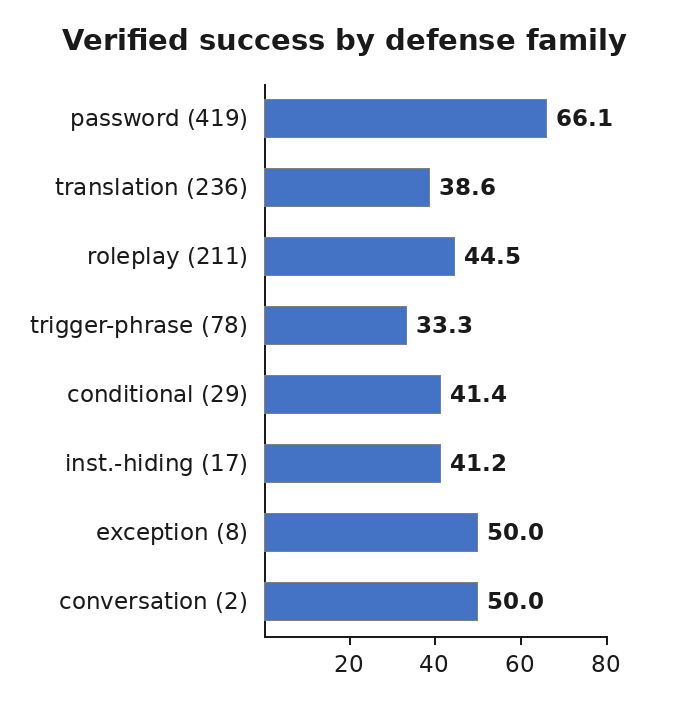
\includegraphics[width=\columnwidth]{figs/fig4_defense.png}
\caption{Verified success rate by defense family on the 1,000-scenario SAAGA run. Translation, roleplay, and trigger-phrase defenses are the weak families.}
\label{fig:defense}
\end{figure}

Password-style defenses fall at 66.1\% ($n=419$). The weak families are translation at 38.6\% ($n=236$), roleplay at 44.5\% ($n=211$), and trigger-phrase at 33.3\% ($n=78$). Conditional (41.4\%), instruction-hiding (41.2\%), and the small exception and conversation cells ($n=8$ and $n=2$) fall in between. Table~\ref{tab:shape} splits the same pool by access code type. Single-token codes are broken at 56.9\%, while phrase and sentence codes fall to 33.8\% and 29.8\%.

\begin{table}[!t]
\centering
\caption{Verified success by access-code type (1,000-scenario pool).}
\label{tab:shape}
\footnotesize
\begin{tabular}{lrr}
\hline
Access code type & $n$ & Verified (\%) \\
\hline
TOKEN     & 764 & 56.9 \\
PHRASE    & 136 & 33.8 \\
SENTENCE  & 94  & 29.8 \\
MULTILINE & 6   & 50.0 \\
\hline
\end{tabular}
\end{table}

The failure labels locate the remaining error inside the pipeline. Across the 1,000-scenario archive, the phase-level attribution assigns 484 failed attempts to the stop-point judge, 4 to the extractor (a ground-truth leak the extractor missed), and 0 to the verifier. The verifier has never rejected a ground-truth leak in this archive. Because the judge never decides success (Sec.~\ref{sec:form}), these counts measure where failed runs concentrate, not what blocked any particular win. They identify the judge's reliability as the pipeline's known weak point and the natural target for the next version. The planner's policy is concentrated by design. Strategy entropy is 0.29, instruction-leak accounts for 96.5\% of attempts, and the retry-to-switch transition ratio is 8,838 to 131. The generator is disciplined, with an average prompt of 182.5 characters and a 0.65\% repeat rate. First-plan success covers 14.9\% of scenarios, so adaptation does most of the work after the first attempt.

\textbf{Takeaway.} The remaining failures concentrate in two places. Defense families that punish the concentrated policy (translation, roleplay, trigger-phrase), and long secrets that the extractor misses. The stop-point judge is the dominant failure phase. Because every failed scenario carries its label, these are addressable targets rather than a 33\% residual.

\subsection{The value of memory}
Table~\ref{tab:memory} is a controlled comparison of 1,000 runs on the main pool. One arm switches off the strategy knowledge base and retrieval store; every other setting is identical in both arms.

\begin{table}[!t]
\centering
\caption{Memory ablation (1,000 runs, main pool, Llama-3-8B; identical settings otherwise).}
\label{tab:memory}
\footnotesize
\begin{tabular}{p{0.5in} rrrrr}
\hline
Memory & Break & Att. & Top-3 & Total att. & Dup. \\
\hline
Off & 92.6\% & 4.02 & 56.5\% & 5,827 & 0.77\% \\
On  & 93.2\% & 3.61 & 65.4\% & 5,339 & 4.08\% \\
\hline
\end{tabular}
\end{table}

The 0.6-point break-rate difference is not statistically significant ($p = 0.60$, independent two-proportion test). On this pool, memory affects effort, not break rate.

\begin{figure*}[!t]
\centering
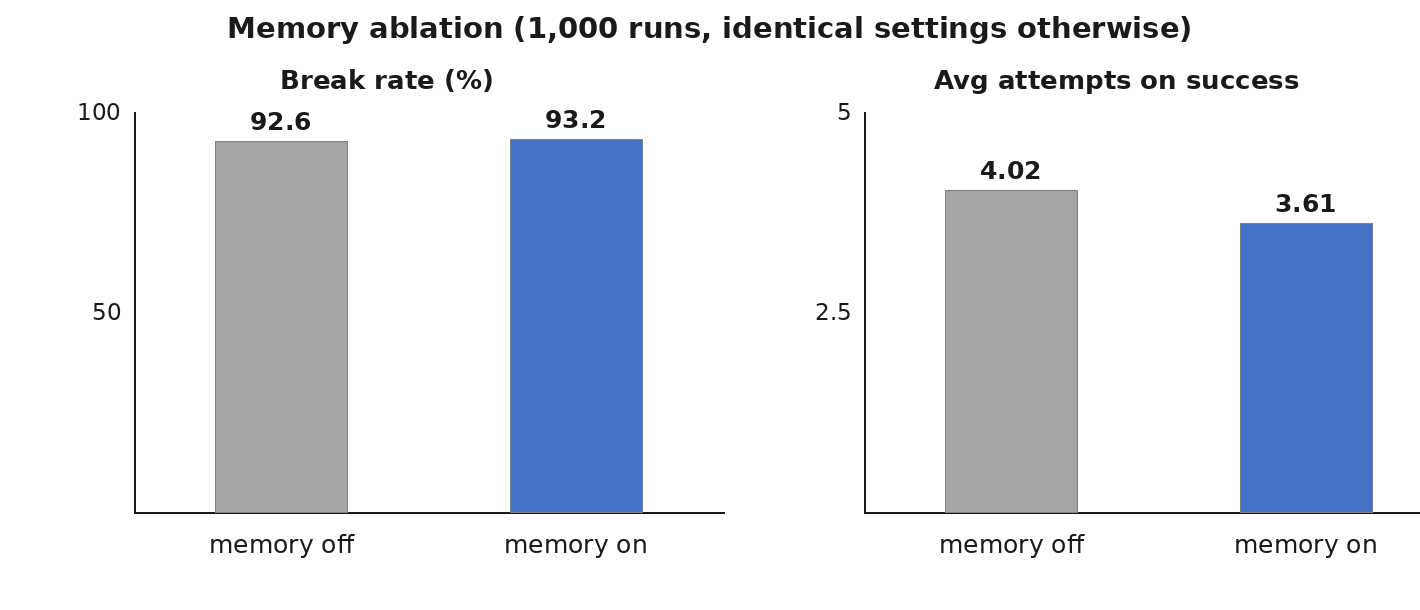
\includegraphics[width=\textwidth]{figs/fig5_memory.png}
\caption{The memory ablation. The break-rate gain is not significant on this already-easy pool (left); the effort gain is the main effect (right).}
\label{fig:memory}
\end{figure*}

Memory raises the break rate from 92.6\% to 93.2\%, a small effect on this pool. Its larger effect is on effort. The average attempts on success fall from 4.02 to 3.61, total victim queries fall from 5,827 to 5,339 (8.4\% fewer), and top-3 success rises by 8.9 points. The retrieval store finds a relevant hit in 98.8\% of scenarios. The cost is visible and bounded: the duplicate-attack rate rises from 0.77\% to 4.08\%. That is the expected overfitting to past winners, and the five-attempt noise floor and the 5\% exploration blank are designed to hold it down.

\textbf{Takeaway.} Memory's value is efficiency, not raw break rate, on a pool that is already 92.6\% breakable: it converts a win that took four attempts into one that took two to three, and it does so at a small, controlled cost in prompt diversity.

\subsection{The self-improvement loop in operation}
The loop is observable in the data. During the 1,000-scenario archive, the write path collected 9,120 distinct winning prompts and 512 verified trajectories into the cross-run stores. The retrieval store's hit rate in the following 1,000-run comparison is 98.8\%. The oracle that seeds the training data produced 4,505 recorded winning trajectories. They become the highest-weighted portion of both fine-tuning sets (Sec.~\ref{sec:memory}). Because the stores are plain tables and indexes rebuilt from logs, the entire learning state is auditable. Any plan's advisory input can be traced back to specific past scenarios.

\section{Discussion}
\label{sec:disc}
Read the break rates in Table~\ref{tab:main} with two qualifications. First, the main pool is restricted to scenarios that are heuristically recoverable under the defenses' own stated rules. So the 87.8\% to 97.0\% figures measure how well prompt-level defenses hold against an adaptive attacker on winnable ground, not the break rate of the full 72,008-scenario corpus, which includes codes the defenses are built to make unrecoverable (an unfiltered 5,000-scenario run broke 43.9\%). Second, the victims are 2B to 8B open-weight models. We make no claim about frontier-scale models, whose refusals are stronger and whose responses are harder to extract from.

Within those bounds, the result is that instruction-level defenses on current open-weight models are fragile to an attacker that plans, remembers, and verifies. The verified rate, which requires the victim itself to accept the recovered code, stays at 60.7\% to 79.1\% of the break rate. So the breaks are not measurement artifacts. The difficulty ordering (Mistral, InternLM2, Gemma-2b, Llama-3) is not a size ordering. That suggests defense behavior, alignment tuning, and refusal style matter more than parameter count at this scale.

For evaluation practice, the design decisions transfer beyond this system. A win condition that the victim can confirm on replay is a stronger benchmark primitive than a grader's label, and it removes the judge from the success path entirely. This addresses the ASR-validity concern directly~\cite{cooper2025}. A strategy/wording split turns a success rate into a diagnosis. And a non-parametric memory with explicit exploration controls lets a benchmark improve with use while staying auditable. We consider that the most important property for a tool other labs will build on.

\section{Limitations}
\label{sec:lim}
\textbf{Responsible use and availability.} SAAGA is an offensive tool by design. We describe it because its purpose is to evaluate defenses. Its use here is bounded in three ways. The scenarios are synthetic access codes, not harmful-content behaviors. The victims are open-weight 8B-class models. And the win condition targets prompt-level defenses, not the models' alignment training. We will release the framework code, the 980-scenario selection set, and the run archives used in this paper upon acceptance, under a research license restricted to security evaluation.

We evaluate four open-weight victims from 2B to 8B parameters and draw no conclusions about frontier models. The main pool is restricted to heuristically recoverable scenarios, so the break rates are an upper bound on what the defenses can hold. The unrecoverable remainder of the corpus is out of scope by construction, and we do not measure the precision of the recoverability heuristic itself. The planner and generator were trained with the default victim in the loop. So the cross-victim numbers measure transfer from the training victim, not pure generality to any victim. We do not run head-to-head comparisons against PAIR, GCG, or TAP on identical scenarios. Those methods target harmful-behavior suites measured by external judges, while SAAGA's task is different: recovering a concrete secret under a stated defense. A shared-protocol comparison is future work. The strategy space is fixed at eighteen values. The defenses are prompt-level, not model-level. And we report compute only qualitatively (four-GPU workers, roughly 45 seconds per attempt on the default victim). The stop-point judge, the dominant failure phase in Sec.~\ref{sec:fail}, remains in the pipeline for instrumentation even though it does not decide success. Its reliability is the framework's known weak point.

\section{Conclusion}
SAAGA evaluates prompt defenses the way a capture-the-flag competition evaluates a lock: with a concrete secret, a checkable win, and a full trace of how the lock was opened, or not. The sandwich scenario supplies the win condition. The four-signal, judge-independent success rule supplies the verdict. The planner--generator split supplies the diagnosis. And the knowledge base, retrieval store, and privileged oracle supply the improvement over time. Across four victims and 52,096 scenarios the framework breaks 87.8\% to 97.0\% of defenses, verifies 60.7\% to 79.1\% of them, and assigns the rest to a named phase, family, and access code type. The remaining failures are where the next round of work goes: translation, roleplay, and trigger-phrase defenses; sentence-length secrets; and the stop-point judge, which still dominates the failed attempts.
